\documentclass[12pt, a4paper]{article}


\usepackage[colorlinks=true,linkcolor=black,anchorcolor=black,citecolor=black,urlcolor=black]{hyperref}
\usepackage{graphicx}
\usepackage{amsmath}
\usepackage{algorithm}
\usepackage{algpseudocode}
\usepackage[margin=3cm]{geometry}
\usepackage{algcompatible}
\usepackage[utf8]{inputenc}
\usepackage{url}


\begin{document}
\begin{titlepage}
	\centering
	\vspace*{0.5 cm}
	\begin{center}    \textsc{\Large Concordia University}\\[2.0 cm]	\end{center}
	\textsc{\Large  SOEN 6011 - Software Engineering Processes }\\[0.5 cm]
	\begin{center} \textsc{\Large Summer 2022} \end{center}
	
	\vspace{15mm}
	
	{ \huge \textbf {ETERNITY}}\\[0.2 cm]
	{ \large \textbf{FUNCTION (F5) : $ab^x$}}
	
	\vspace{90mm}	
	\begin{center}   
		{\large \textbf{Harshkumar Nileshkumar Patel}  }\\[0.2 cm]
		{\large Student ID : 40165709 }\\[0.2 cm]
		\vspace{10mm}
		{\large Github Link :- \url{https://github.com/harshp189/SOEN\_6011\_F5}}
	\end{center}
		
\end{titlepage}
\tableofcontents
\newpage

\section{Problem 1 : Introduction}
\subsection{Description}

F5 : $ab^x$ is an exponential function, where a is a constant value, $a \ne 0$ and it represents starting (initial) value , $b$ is called base and is a positive real number, $b > 1$, $x$ is called the exponent (power). In this function, $b$ is a constant and $x$ is  independent variable \cite{Exponential Growth and Decay}.

\subsection{Domain}

The domain for exponential function is the set of real numbers. 
\newline $ x \in R $ ,  -$ \infty < x <\infty $ , Domain : $ \{x \mid x \in R $\}

\subsection{Co-Domain}

Co-Domain is the set of all possible function output values.
\newline For the given function , suppose $y = f(x) = ab^x $, then -$ \infty < y <\infty $ , so the range will be $ (-\infty,\infty) $. So the range of the exponential function is $R$, $ y \in R $, where $ x \in R $ , $ b > 0 $.

\subsection{Characteristics}
\begin{itemize}
	\item In exponential function, if $ b > 0 $, then it is known as exponential growth function (increasing function). Its graphical representation shown in the left part of the figure 1.
	\item In exponential function, if $ 0 < b < 1$, then it is known as exponential decay function (decreasing function). Its graphical representation shown in the right part of the figure 1.
	\item Exponential function have horizontal asymptote (i.e function approaches to a imaginary horizontal line but never crosses) at $ Y=0 $ (i.e $ X $ – axis).
	\item They are continuous function.
	\item There is no symmetry in exponential function, so they are neither odd nor even function.
	\item Exponential function is not injective but is surjective \cite{Injectivity and Surjectivity of Exponential Function}.
\end{itemize}

\newpage

\begin{figure}[h]
	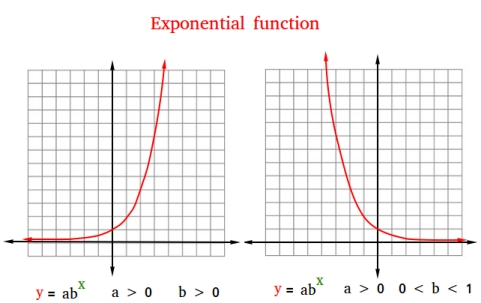
\includegraphics[width=\linewidth]{exponential-function.jpg}
	\caption{Exponential Function Graph (Growth And Decay) \cite{Exponential Function Graph}.}
	\label{fig:exponential function graph (growth and decay)}
\end{figure}

\subsection{Context of Use Model}
\begin{figure}[h!]
	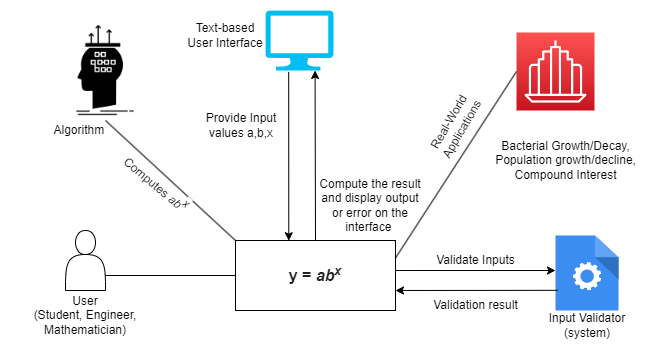
\includegraphics[width=\linewidth]{ContextOfUse.png}
	\caption{Context of Use model diagram in 'Boxes-and-Lines'}
	\label{fig:Context of Use model}
\end{figure}


\newpage

\section{Problem 2 : Requirements}
\subsection{Assumptions}
\begin{enumerate}
	\item{} Assumption 1
	\begin{itemize}
		\item \textbf{ID} : A1
		\item \textbf{Description} : The user should provide input values for all $``a``, ``b`` \hspace{1mm}and \hspace{1mm}``x``$. As  no default values are assumed for the calculation of the function.
	\end{itemize}
	     
	\item{} Assumption 2
	\begin{itemize}
		\item \textbf{ID} : A2
		\item \textbf{Description} : Inputs for the function should be real number and the output of the function is also a real number.
	\end{itemize}
	    
	\item{} Assumption 3
	\begin{itemize}
		\item \textbf{ID} : A3
		\item \textbf{Description} : For large input values which are out of the range, the results are undefined.
	\end{itemize}
	    
\end{enumerate}



\subsection{Requirements}
The Functional and Non-Functional Requirements are expressed using guidelines from the ISO/IEC/IEEE 29148:2018 standard \cite{Requirements Engineering}.
\begin{enumerate}
	\item{} Requirement 1
	\begin{itemize}
		\item \textbf{ID} : REQ1
		\item \textbf{Version} : 1.0
		\item \textbf{Type} : Functional Requirement
		\item \textbf{Priority} : High
		\item \textbf{Difficulty} : Easy
		\item \textbf{Description} : In the exponential function $ ab^x $, the input value a should not be 0 i.e., $ a \neq 0 $ (or else it will result in output of the function to be 0 for every input), also input value of base b must be greater than 1 i.e., $ b > 1 $ (or else if $b = 1 $, it will result in output of the function to be ‘a’ for every input of x).
	\end{itemize}
	    
	\item{} Requirement 2
	\begin{itemize}
		\item \textbf{ID} : REQ2
		\item \textbf{Version} : 1.0
		\item \textbf{Type} : Functional Requirement
		\item \textbf{Priority} : High
		\item \textbf{Difficulty} : Easy
		\item \textbf{Description} : In the exponential function $ab^x$, the input value of base b must not be negative as it will result in complex numbers so $b > 0$. Also, the input value of $x$ must be any real number. i.e $x \in R$.
	\end{itemize}
	    
	    
	\item{} Requirement 3
	\begin{itemize}
		\item \textbf{ID} : REQ3
		\item \textbf{Version} : 1.0
		\item \textbf{Type} : Functional Requirement
		\item \textbf{Priority} : High
		\item \textbf{Difficulty} : Medium
		\item \textbf{Description} : The system must take input values of a, b and x from the users and return the output of $ab^x$ function. For example, if $ a = 2, b = 3 , x = 2,$ the output should be $ 18 $.
	\end{itemize}
	        
	    
	\item{} Requirement 4
	\begin{itemize}
		\item \textbf{ID} : REQ4
		\item \textbf{Version} : 1.0
		\item \textbf{Type} : Functional Requirement
		\item \textbf{Priority} : High
		\item \textbf{Difficulty} : Medium
		\item \textbf{Description} : The system must be able to compute the value of the function $ab^x$ when the input value of exponent $x$ is fractional or negative and must handle all the cases.
	\end{itemize}
	        
	\item{} Requirement 5
	\begin{itemize}
		\item \textbf{ID} : REQ5
		\item \textbf{Version} : 1.0
		\item \textbf{Type} : Functional Requirement
		\item \textbf{Priority} : High
		\item \textbf{Difficulty} : Easy
		\item \textbf{Description} : If the input values are not of numeric type (real number), the system must not accept it and display the error and ask for numeric values as input.
	\end{itemize}
	    
	\item{} Requirement 6
	\begin{itemize}
		\item \textbf{ID} : REQ6
		\item \textbf{Version} : 1.0
		\item \textbf{Type} : Functional Requirement
		\item \textbf{Priority} : High
		\item \textbf{Difficulty} : Easy
		\item \textbf{Description} : If any of the input values a, b or x are not provided by the user, the system should not accept that input and ask user to provide the missing values. 
	\end{itemize}
	    
	 
	    
	     
	\item{} Requirement 7
	\begin{itemize}
		\item \textbf{ID} : REQ7
		\item \textbf{Version} : 1.0
		\item \textbf{Type} : Non-Functional Requirement
		\item \textbf{Priority} : High
		\item \textbf{Difficulty} : Medium
		\item \textbf{Description} : The computation of the function must be performed within some desired time to provide better performance.
	\end{itemize}
	    
	\item{} Requirement 8
	\begin{itemize}
		\item \textbf{ID} : REQ8
		\item \textbf{Version} : 1.0
		\item \textbf{Type} : Non-Functional Requirement
		\item \textbf{Priority} : High
		\item \textbf{Difficulty} : Medium
		\item \textbf{Description} : The text-based user interface must be user-friendly and appropriate error messages should be displayed for the corresponding error by the system.
	\end{itemize}
	    
	\item{} Requirement 9
	\begin{itemize}
		\item \textbf{ID} : REQ9
		\item \textbf{Version} : 1.0
		\item \textbf{Type} : Non-Functional Requirement
		\item \textbf{Priority} : High
		\item \textbf{Difficulty} : Medium
		\item \textbf{Description} : The system must be maintainable, i.e, it should be easy to modify the existing system or add any new features/functionality over time.
	\end{itemize}
	    
\end{enumerate}

\newpage

\section{Problem 3 : Algorithms}

Two algorithms (Algorithm 1 and Algorithm 2) have been selected for \newline
implementing the function $y = ab^x $. The pseudocode for each of the algorithm is provided in this section followed by their detailed description and the advantages as well as the disadvantages of each approach are discussed later.

\subsection{Pseudocode format}
\begin{figure}[h]
	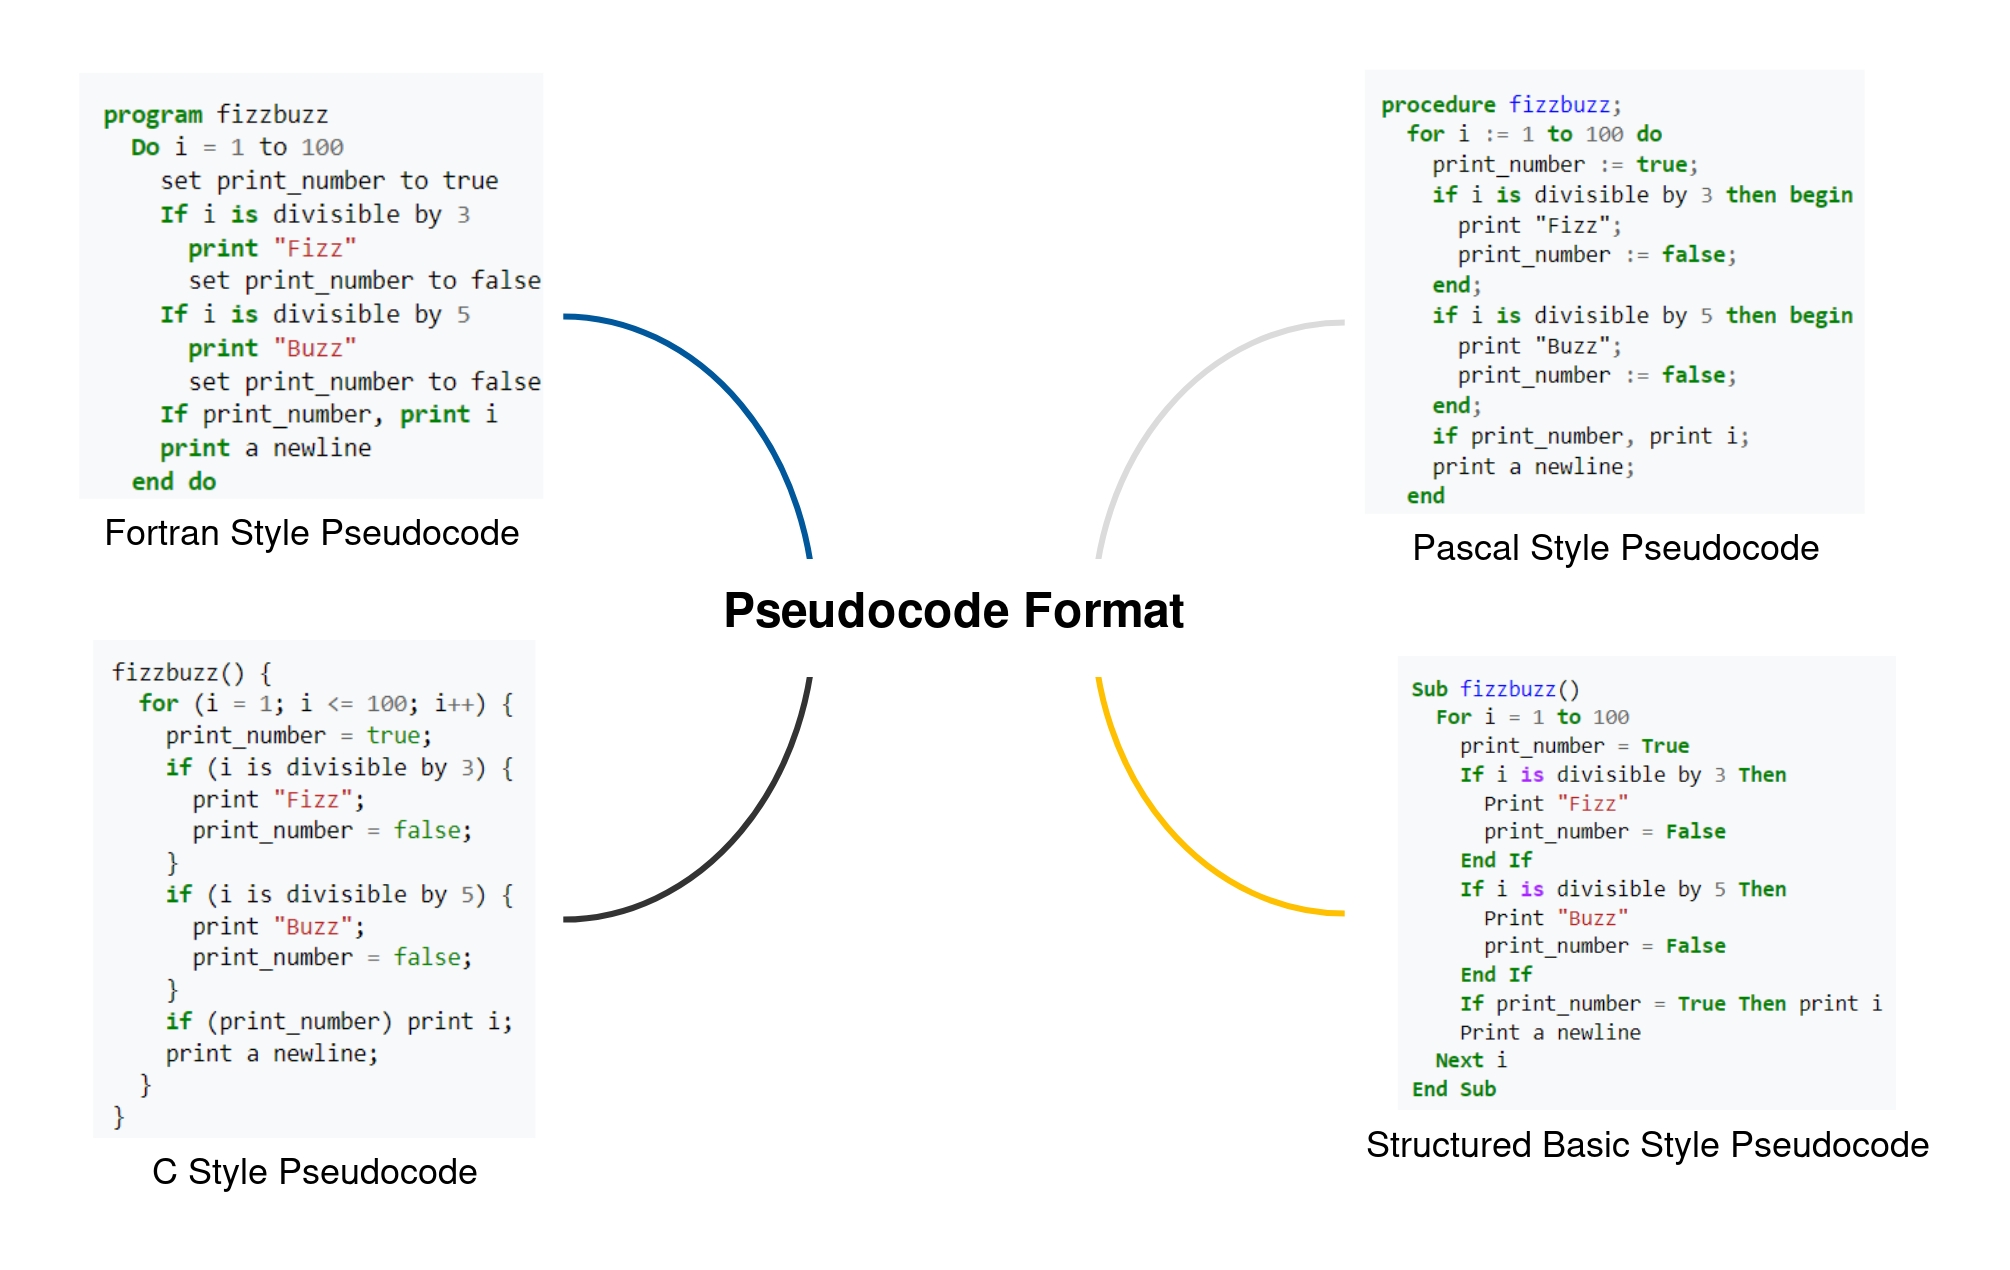
\includegraphics[width=15cm,height=9cm]{Pseudocode Format.jpg}
	\caption{Mindmap of different pseudocode formats}
	\label{fig:Mindmap of different pseudocode formats}
\end{figure}
\noindent
As shown in the figure, there are four types of pseudocode formats, Fortran Style, Pascal Style, C Style, Structured Basic Style for describing the pseudocode for the algorithms \cite{Pseudocode}, I have selected the Structured Basic Style Pseudocode format as LaTeX provides support for this kind of format for typesetting algorithms by the help of several packages, I have used the algpseudocode package and algorithm package.

\newpage
\subsection{Algorithms and Pseudocode}
\begin{algorithm}[hbt!]
	\caption{Iterative-Exponent(a,b,x)}\label{alg:one}
	
	\hspace*{\algorithmicindent} \textbf{Input : }double number $a,b,x$ \\
	\hspace*{\algorithmicindent} \textbf{Output : }value of the function $ab^x$ represented by double number result
	\begin{algorithmic}[1]
		\STATE $temp \gets 1$
		\WHILE{$x > 0$}
		\STATE $temp \gets temp \times b$
		\STATE $x \gets x - 1$
		\ENDWHILE
		\STATE $result \gets a \times temp$
		\STATE return $result$
	\end{algorithmic}
\end{algorithm}

\noindent
In this algorithm, the iterative approach is used for calculation of the given function, $ab^x$, Initially a temporary  variable called $temp$ is initialized to 1 and to calculate $b^x$, While loop is used for all the values of $x$ (exponent) and in each iteration, $temp$ is multiplied by $b$ (base) and the value of $x$ is decremented by 1. The loop continue until the exponent value $x$ reaches to 0. At last, $a$ is multiplied with the $temp$ value $(a*b^x)$ and the output is obtained in the result and it is returned.

\vspace{90mm}


\begin{algorithm}[hbt!]
	\caption{Recursive-Exponent(a,b,x)}\label{alg:two}
	
	\hspace*{\algorithmicindent} \textbf{Input : }double number $a,b,x$ \\
	\hspace*{\algorithmicindent} \textbf{Output : }value of the function $ab^x$ represented by double number result
	\begin{algorithmic}[1]
		\STATE $temp \gets recursive\_power(b,x)$
		\STATE $result \gets a \times temp$
		\STATE return $result$
	\end{algorithmic}
\end{algorithm}

\newpage


\begin{algorithm}[hbt!]
	\renewcommand{\thealgorithm}{2.1}
	\caption{recursive\_power(b,x)}\label{alg:two}
	
	\hspace*{\algorithmicindent} \textbf{Input : }double number $b,x$. \\
	\hspace*{\algorithmicindent} \textbf{Output : }value of $b^x$ will be returned.
	\begin{algorithmic}[1]
		\IF{$x \neq (Integer) x $}
		\STATE return $ fraction\_power(b,x) $
		\ENDIF
		\STATE $helper \gets recursive\_power(b,x/2)$
		\IF{$x < $ 0}
		\STATE $ b  \gets $ 1.0/$ b $
		\STATE $ x  \gets  - x $
		\IF{$x$ mod 2 = 0}
		\STATE return $helper \times helper$
		\ELSE
		\STATE $x \gets x - 1$
		\STATE return $helper \times helper \times b$
		\ENDIF
		\ELSIF{$x$ = 0}
		\STATE return $1.0$
		\ELSIF{$x$ = 1}
		\STATE return $b$
		\ELSIF{$x$ mod 2 = 0}
		\STATE return $helper \times helper$
		\ELSE
		\STATE $x \gets x - 1$
		\STATE return $helper \times helper \times b$
		\ENDIF
	\end{algorithmic}
\end{algorithm}

\noindent
In this algorithm, the recursive approach using optimized divide and conquer strategy is used for the calculation of the given function $ab^x$ \cite{Recursive Power Function}. $recursive\_power(b,x)$ algorithm is used for calculating the value of $b^x$, the recursive call to the function with value base $b$ and $x = x/2$ i.e $recursive\_power(b,x/2)$ is stored in helper, so that it needs to be computed just once and can be used later on. If the value of exponent $x$ is fractional, it is checked and $fraction\_power(b,x)$ will compute all the power values of such exponents. For negative value of exponent, value of base $b$ is reciprocated and that of exponent $x$ is negated and on the basis of the parity, the algorithm performs the computation. In the base case, if the value of $x$ is 0, value $1$ is returned, otherwise, if $x=1$, value $b$ is returned, if the exponent is divisible by $2$, the algorithm recurses on $(helper * helper)$ and for odd value of exponent, the value of exponent is decremented by $1$ and then it recurses on $(helper * helper * b)$,  At last, $a$ is multiplied with the returned value from $recursive\_power(b,x)$ and the output is obtained in the $result$, and it is returned.

\newpage
\begin{algorithm}[hbt!]
	\renewcommand{\thealgorithm}{2.2}
	\caption{fractional\_power(b,x)}\label{alg:two}
	
	\hspace*{\algorithmicindent} \textbf{Input : }double number $b,x$. \\
	\hspace*{\algorithmicindent} \textbf{Output : }value of $b^x$ will be returned.
	\begin{algorithmic}[1]
		\STATE $e \gets 2.7182818284590$
		\STATE $exponentValue \gets 0$
		\STATE $iterations \gets 20$
		\STATE $logValue \gets logarithm\_calculator(b)$
		\STATE $eValueX \gets (x \hspace{1mm} * \hspace{1mm} logValue)$
		\STATE $eValueR \gets eValueX - (int)\hspace{1mm}eValueX$
		\WHILE{$iterations >= 0$}
		\STATE $powerValue \gets recursive\_power(eValueR , iterations) $
		\STATE $factorialValue \gets factorial\_calculator(iterations)$ 
		\STATE $exponentValue \gets exponentValue + (powerValue / factorialValue)$
		\STATE $iterations \gets iterations - 1$
		\ENDWHILE
		\STATE $eValueN \gets recursive\_power(e, (int) \hspace{1mm} eValueX)$
		\STATE $eFinalValue \gets exponentValue \hspace{1mm}*\hspace{1mm} eValueN$
		\STATE return $eFinalValue$
	\end{algorithmic}
\end{algorithm}
\vspace*{-.4cm}
\begin{algorithm}[hbt!]
	\renewcommand{\thealgorithm}{2.3}
	\caption{logarithm\_calculator(n)}\label{alg:two}
	
	\hspace*{\algorithmicindent} \textbf{Input : }double number $n$. \\
	\hspace*{\algorithmicindent} \textbf{Output : }natural logarithmic value of n $ln(n)$ will be returned.
	\begin{algorithmic}[1]
		
		\STATE $iterations \gets 100$
		\STATE $logValue \gets 0 $
		\IF{$n < $ 0}
		\STATE $n \gets -n$
		\ENDIF
		\STATE $baseValue \gets (n - 1) / (n + 1) $
		
		\WHILE{$iterations > 0$}
		\IF{$iterations$ mod $2 \neq 0$}
		\STATE $logValue \gets logValue + recursive\_power(baseValue , iterations) / iterations $
		\ENDIF
		\STATE $iterations \gets iterations - 1$
		\ENDWHILE
		\STATE return $logValue * 2$
		
	\end{algorithmic}
\end{algorithm}

\begin{algorithm}[hbt!]
	\renewcommand{\thealgorithm}{2.4}
	\caption{factorial\_calculator(n)}\label{alg:two}
	
	\hspace*{\algorithmicindent} \textbf{Input : }double number $n$. \\
	\hspace*{\algorithmicindent} \textbf{Output : }factorial value of $n$ will be returned.
	\begin{algorithmic}[1]
		
		\IF{$n = $ 0}
		\STATE return $1$
		\ENDIF
		\STATE return $ (n * factorial\_calculator(n-1)) $
		
	\end{algorithmic}
\end{algorithm}



\newpage
\noindent
Algorithm $fractional\_power(b,x) $ helps in finding the power of any fractional exponent, the given exponent and base are converted as, $b^x = (e^{ln(b)})^x = e^{xln(b)} $ \cite{Algorithms}, where the natural logarithm value for b is computed using the $logarithm\_calculator(n) $ algorithm. Finally, for the computation of $e^{xln(b)} $ , $(eValueX)$ it is splitted into $e^r$ $(eValueR)$ and $e^n$ $(eValueN)$,

$e^{xln(b)} $ = $e^r * e^n $ 

\noindent
where $e^r$ is computed in the while loop by calculating numerator(powerValue) by using $recursive\_power$ , passing $eValueR$ as base and $iteration \hspace{1mm} number$ as exponent and the denominator is the factorial value of the iteration number obtained using the $factorial\_calulcator(n)$ algorithm, numerator and denominator are divided and their result is stored in the $exponentValue$ which is returned after completion of all the given number of iterations. Similarly $e^n$ $(eValueN)$ is computed by using $recursive\_power$, passing the value of $e$ as base and $(int) eValueX$ as the exponent, at last both $exponentValue$ and $eValueN$ are multiplied and their product is returned as the final value.
 
 
\noindent
Algorithms 2.1, 2.2, 2.3 and 2.4 are defined to help in the computation of the main Algorithm 2.

\subsection{Advantages and Disadvantages}



\subsubsection{Algorithm 1}
Iterative Approach

Advantages:
\begin{enumerate}
	\item {Iterative algorithms are simple and easy to develop; they can be easily understood by the reader.}
	\item {In Iterative approach there is no overhead of function calls and they do not use stack memory and hence don’t suffer from stack overflow.}
	          
\end{enumerate}

Disadvantages:
\begin{enumerate}
	\item {Some iterative algorithms are slower when compared to other approaches, Algorithm 1 which was described previously has time complexity of $O(n)$ , so for larger inputs it is inefficient.}
	\item {If the termination condition of control variable is not defined properly, it may lead to infinite loop.}
	          
\end{enumerate}
\newpage
\subsubsection{Algorithm 2}
Recursive Approach 

Advantages:
\begin{enumerate}
	\item {Recursive Algorithms have less time complexity for certain problems;  Algorithm 2 which was described previously has time complexity of $O(logn)$ which is better than that of Algorithm 1.}
	\item {Recursive Algorithms are very useful in situations where particular solution is to be applied repeatedly \cite{Advantages and Disadvantages of Recursion}.}
	          
\end{enumerate}

Disadvantages:
\begin{enumerate}
	\item {Recursion is more difficult to understand in some algorithms and tracing them is difficult}
	\item {Recursive algorithms utilize too much memory and when the base case is not defined properly it may lead to infinite loop or crashing of the CPU.}
	          
\end{enumerate}

\subsection*{Decision}
\noindent
Algorithm 2 follows optimized divide and conquer approach and provides $ O(logn) $ time complexity as well as space complexity, so the recursive algorithm is faster in comparison to Algorithm 1 which provides time complexity of $ O(n) $. Recursive approach is better when the problem can be divided into smaller problems which are repeated and the function $ ab^x $, can be partitioned into sub problems so it is better to choose the recursive algorithm. Using recursive strategy in the optimized divide and conquer approach leads to reduction of problem size at each step and uses less time for the computation than the iterative approach. Also, all the cases like negative exponent, fractional exponent are efficiently handled by the recursive algorithm. As a result, I have opted to use Algorithm 2(recursive algorithm) for the implementation of the function $ ab^x $ as it is a better option as compared to Algorithm 1(iterative algorithm).

\newpage


\section{Problem 4 }
\subsection{Debugger}
\subsubsection{Description}
Debugging provides the facility for identifying and eliminating bugs, errors present in the program. This process can help in tracing the reasons behind the improper functional behaviour of any program. For debugging, I have used the IntelliJ debugger tool for java language and it provides support for debugging code in different languages as well by installation of various plugins. IntelliJ debugger allows the facility to run the program step by step and keep a track of the values of the associated variables \cite{IntelliJ Debugger}.

\subsubsection{Advantages : }
\begin{enumerate}
	\item Breakpoints are special kind of markers which when encountered, the debugger temporarily halts the program execution (suspended program state) and it makes easier to analyse and debug those special lines.
	\item It allows to trace the values of the variable throughout the program, such trace would be helpful to identify the points where the incorrect values are assigned to the variables, also it provides information about the status of the threads.
	\item It enables execution of any arbitrary piece of code in the middle of the program's execution as well as throw exceptions to test the functional behaviour of the program under different circumstances. Also allows running multiple debugging sessions at the same time.
	\item IntelliJ debugger provides a feature called stepping tool which provides control over the step-by-step execution of the program and helps in deducing the source of the error.
	\item IntelliJ debugger supports the feature to modify and adjust the parts of code without requiring to termination of the ongoing debugging process, it eliminates the need to modify the values of the variable and run the debugger again from start.
\end{enumerate}

\subsubsection{Disadvantages : }
\begin{enumerate}
	\item With the help of debugger, the location of the problem can be identified but the logical error associated with it cannot be known.
	\item Debugger does not provide insights on design issues as well as structure of the code and there is a learning curve associated with it.
	\item Debugger faces several problems while dealing with multithreading programs. 
\end{enumerate}

\newpage

\begin{figure}[h]
	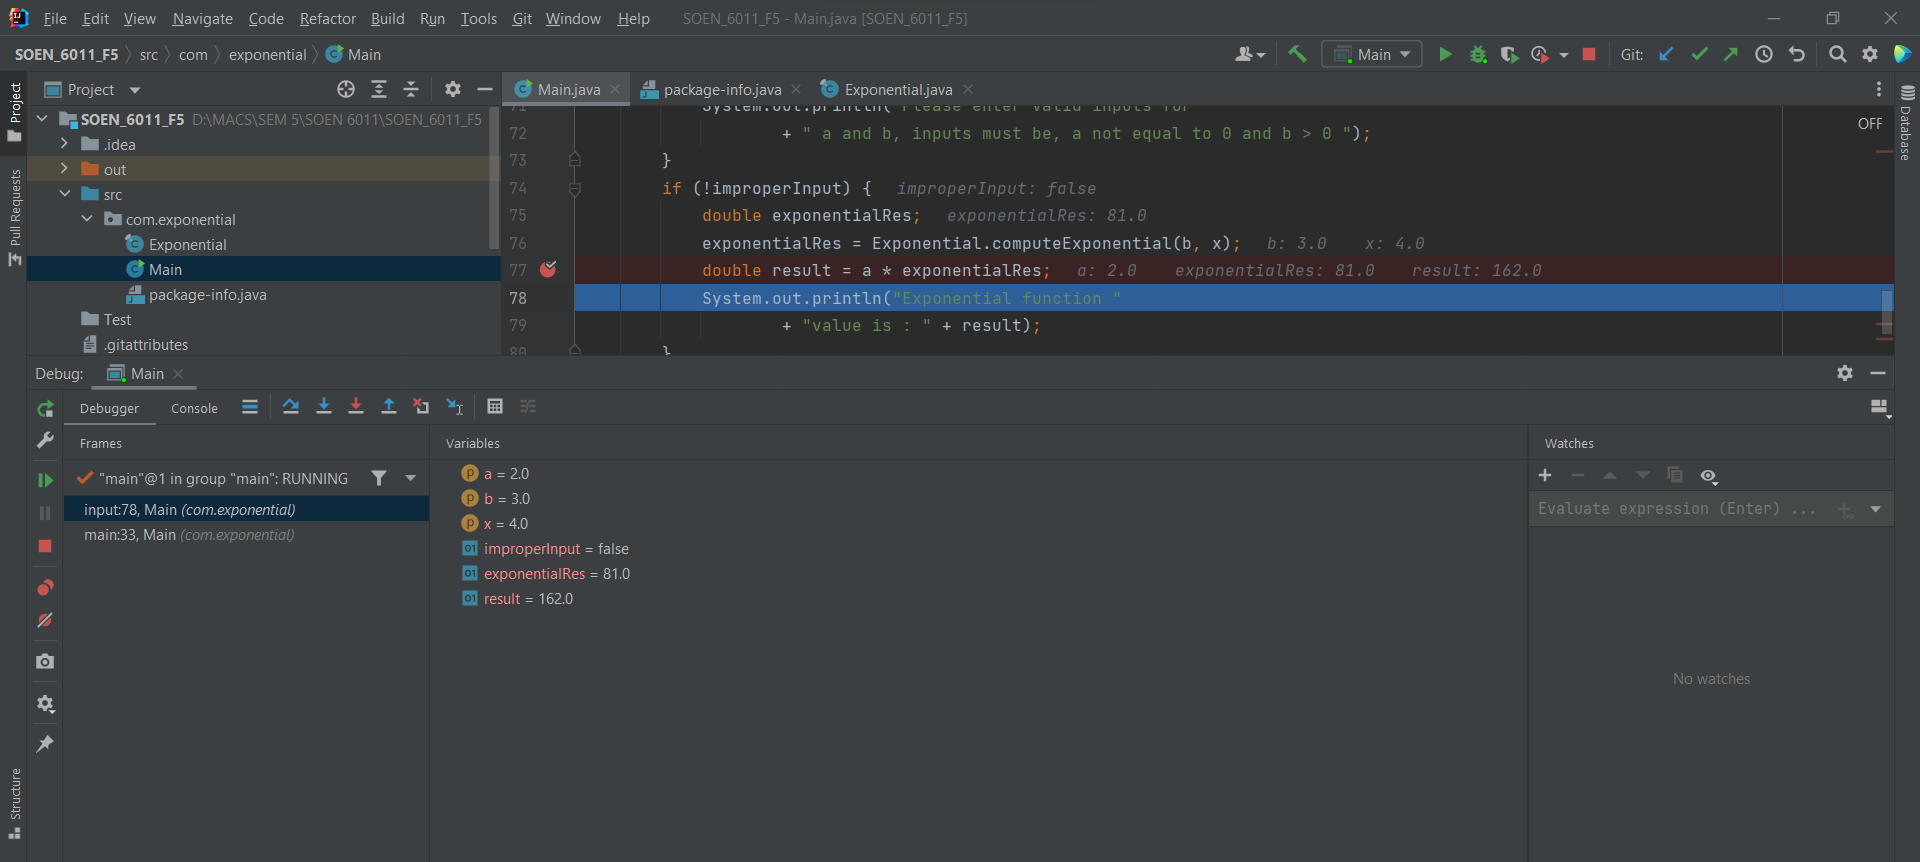
\includegraphics[width=15cm,height=9cm]{debugger-1.png}
	\caption{Debugging computation of exponential function}
	\label{fig:Debugging computation of exponential function}
\end{figure}


\begin{figure}[h!]
	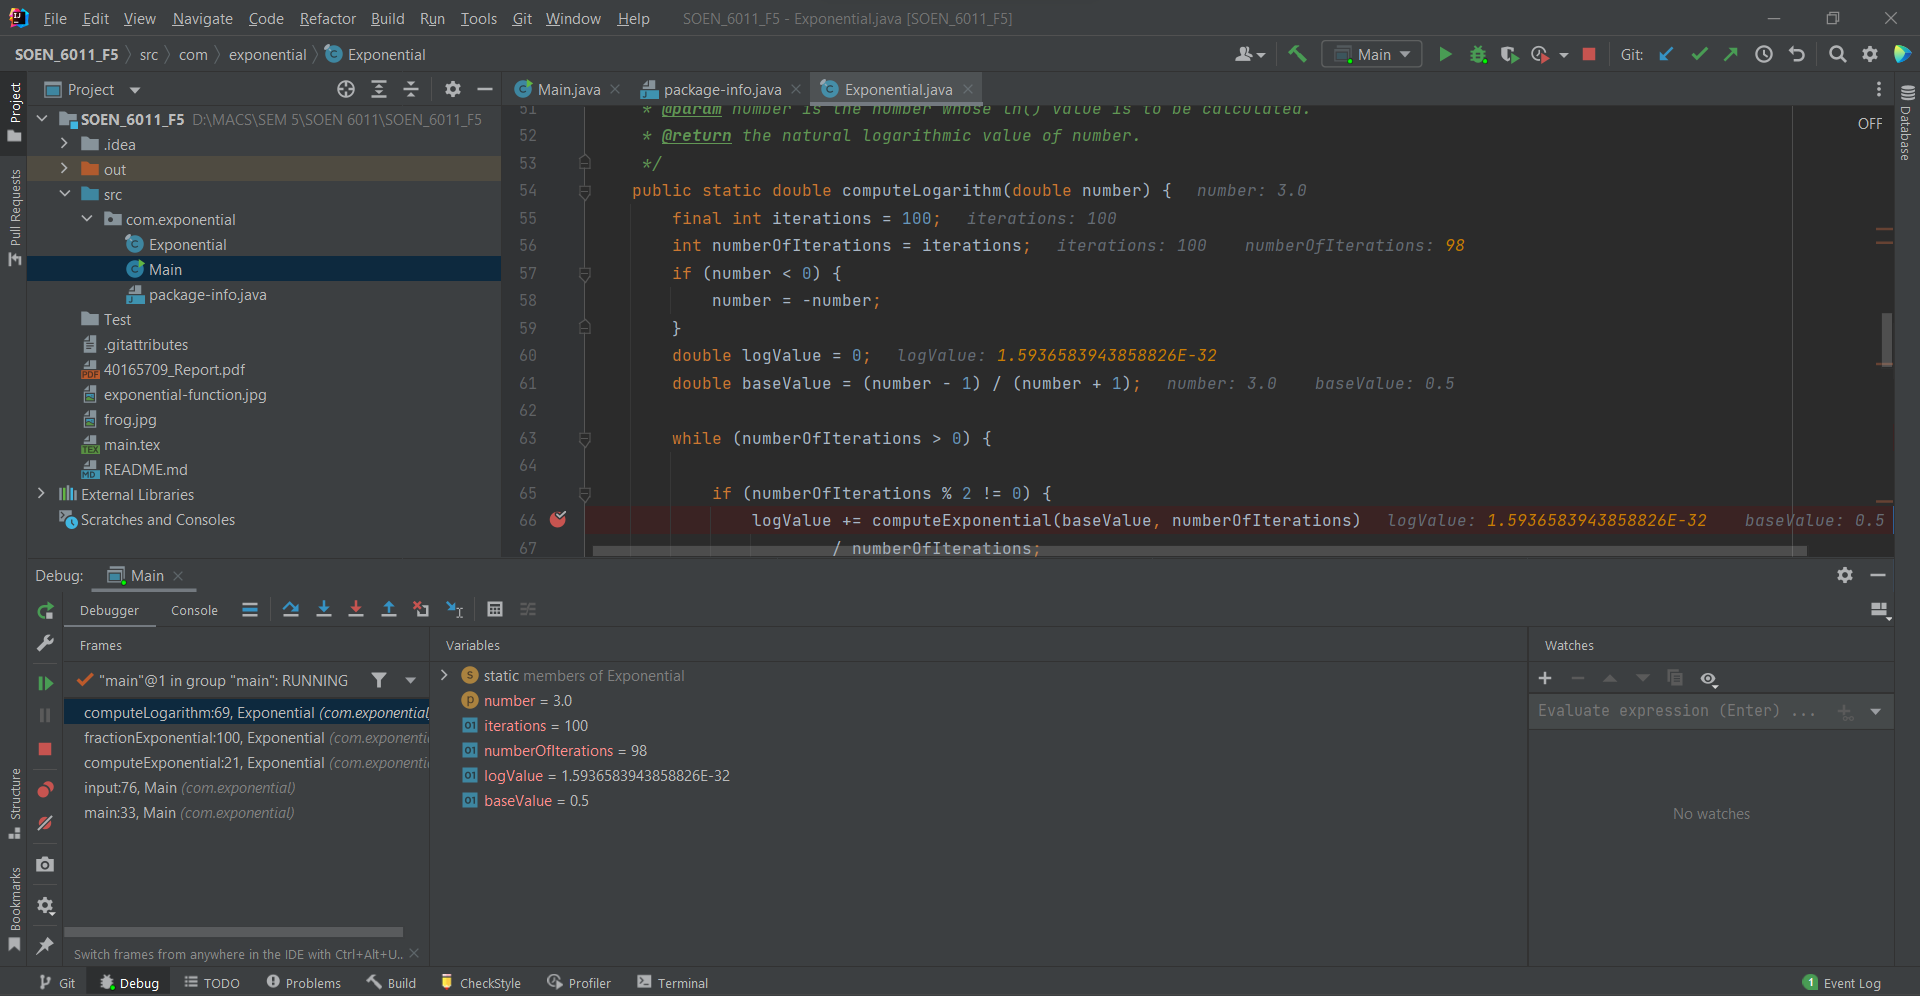
\includegraphics[width=15cm,height=9cm]{debugger-2.png}
	\caption{Debugging computation of fractional exponent value}
	\label{Debugging computation of fractional exponent value}
\end{figure}

\newpage

\subsection{Quality Attributes}
This section highlights and describes several efforts made to achieve the desired quality attributes related to the java program \cite{Quality Assurance}.
\begin{enumerate}
	\item \textbf{Efficient} – The program uses recursive algorithm to compute the exponential value and it provides time complexity of $O(logn)$ and it is the same for space complexity due to recursive stack space. It is more efficient and better choice in comparison to other approaches. As a result, the program runs quickly, and the function value is computed within required time window.
	\item \textbf{Maintainable} – The program is partitioned into various methods each responsible for certain kind of computation, I have divided the user interface, error handling part $(Main.java)$ from the core logic part $(Exponential.java)$ related to the calculation of exponential function value. It allows easy modification of features/functionalities as well as adding new ones. It makes the code maintainable.
	\item \textbf{Correctness} – I have designed several test cases to check the program against all the possible values of the base and exponent including invalid inputs, fractional exponent, negative exponents, every test case runs successfully and hence the developed program provides correct results and agrees to the desired specifications.
	\item \textbf{Robust} – Input values are validated as they are entered by the user and all the invalid inputs are rejected. On entering such inputs, the program displays corresponding error message and asks for new valid input values from the user. In this way error handling is performed to avoid any kind of failure. 
	\item \textbf{Usable} – The program provides text-based user interface to the user for entering the values and displays the computed result. The error messages are meaningful and can be easily understood. It provides functionality for user to continue the computation for other values or exit the system. In this way, the program is made user-friendly.
	\item \textbf{Portable} - The program is developed in java language, so it can be executed on other platforms as well as systems without requiring any modifications. 
\end{enumerate}

\newpage
\subsection{Quality review of source code}
To check the pragmatic quality of the code, I have used the Checkstyle tool and installed the Checkstyle plug-in in the IntelliJ IDE. It is a development tool used to ensure that proper coding standards are adhered by the java code. It automates the process of checking the java code and removes the need to manually perform that task. By default, it provides support for Sun code conventions and Google Java style standards. I have checked my java code against the Google Java programming style coding standards \cite{Checkstyle} .

\subsubsection{Advantages : }
\begin{enumerate}
	\item It is highly configurable and provides support to multiple IDEs (IntelliJ, Eclipse) via the plug-in.
	\item Checkstyle can also perform checking for various issues related to formatting and layout of the code.
	\item It allows creation and checking against various user-defined rules according to the project requirements.
	\item Checkstyle displays a panel with all the error/warnings messages related to the violation of the desired coding standards, it also points out the location and provides suggestion to solve it.
	\item Checkstyle is designed as a standalone framework and it is easier to integrate it with other external tools.
\end{enumerate}

\subsubsection{Disadvantages : }
\begin{enumerate}
	\item Checkstyle provides functionality to locate the errors but does not support their automatic correction.
	\item For any large-scale application with large number of lines of code, it becomes difficult for the programmer to analyse and resolve every errors/warning found by Checkstyle.
	\item Checkstyle only checks the code against the coding standards but does not validate the correctness of the java code.
\end{enumerate}

\noindent
Before using the Checkstyle tool there were around 45+ errors related to coding standards  and all of them were solved. The snapshots of error messages in the source code before using Checkstyle tool and after modifying the code according to desired coding standards are attached below. 


\newpage

\begin{figure}[h]
	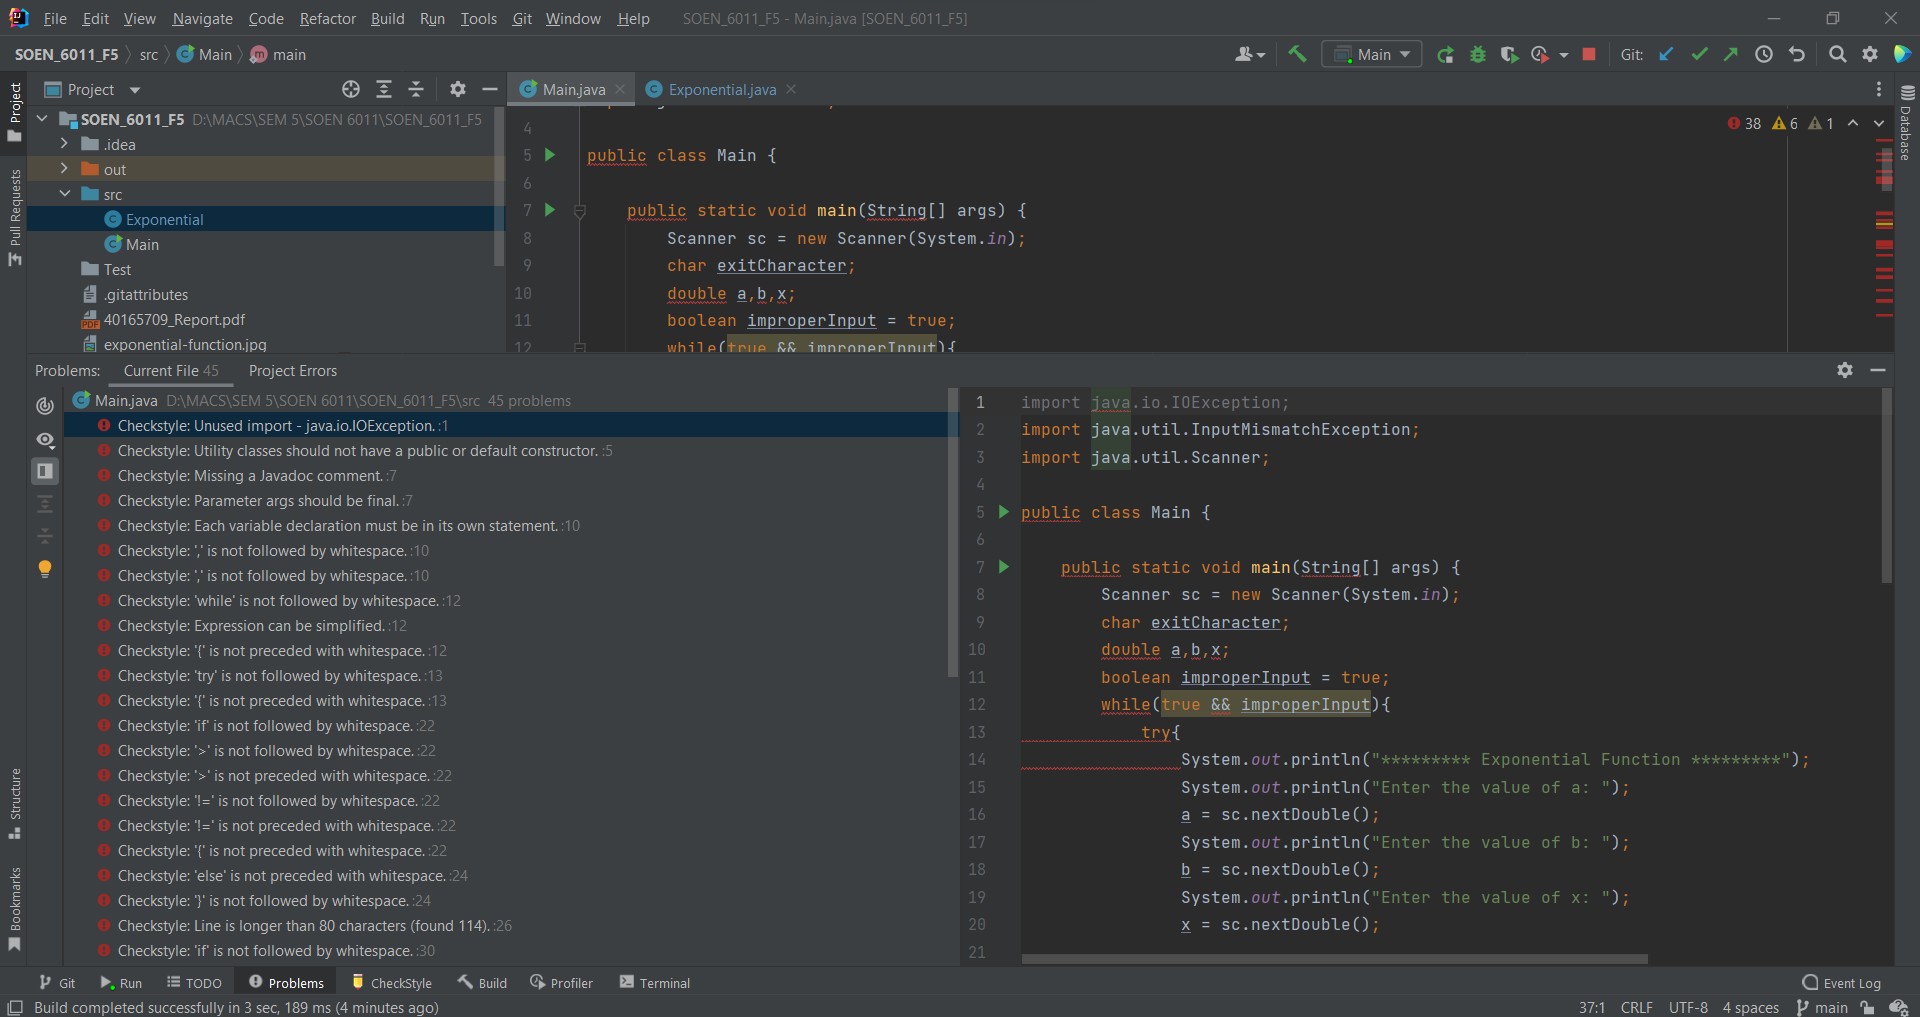
\includegraphics[width=15cm,height=9cm]{CheckStyle(Before).png}
	\caption{Error messages in the source code detected by Checkstyle tool}
	\label{fig:Debugging computation of exponential function}
\end{figure}


\begin{figure}[h!]
	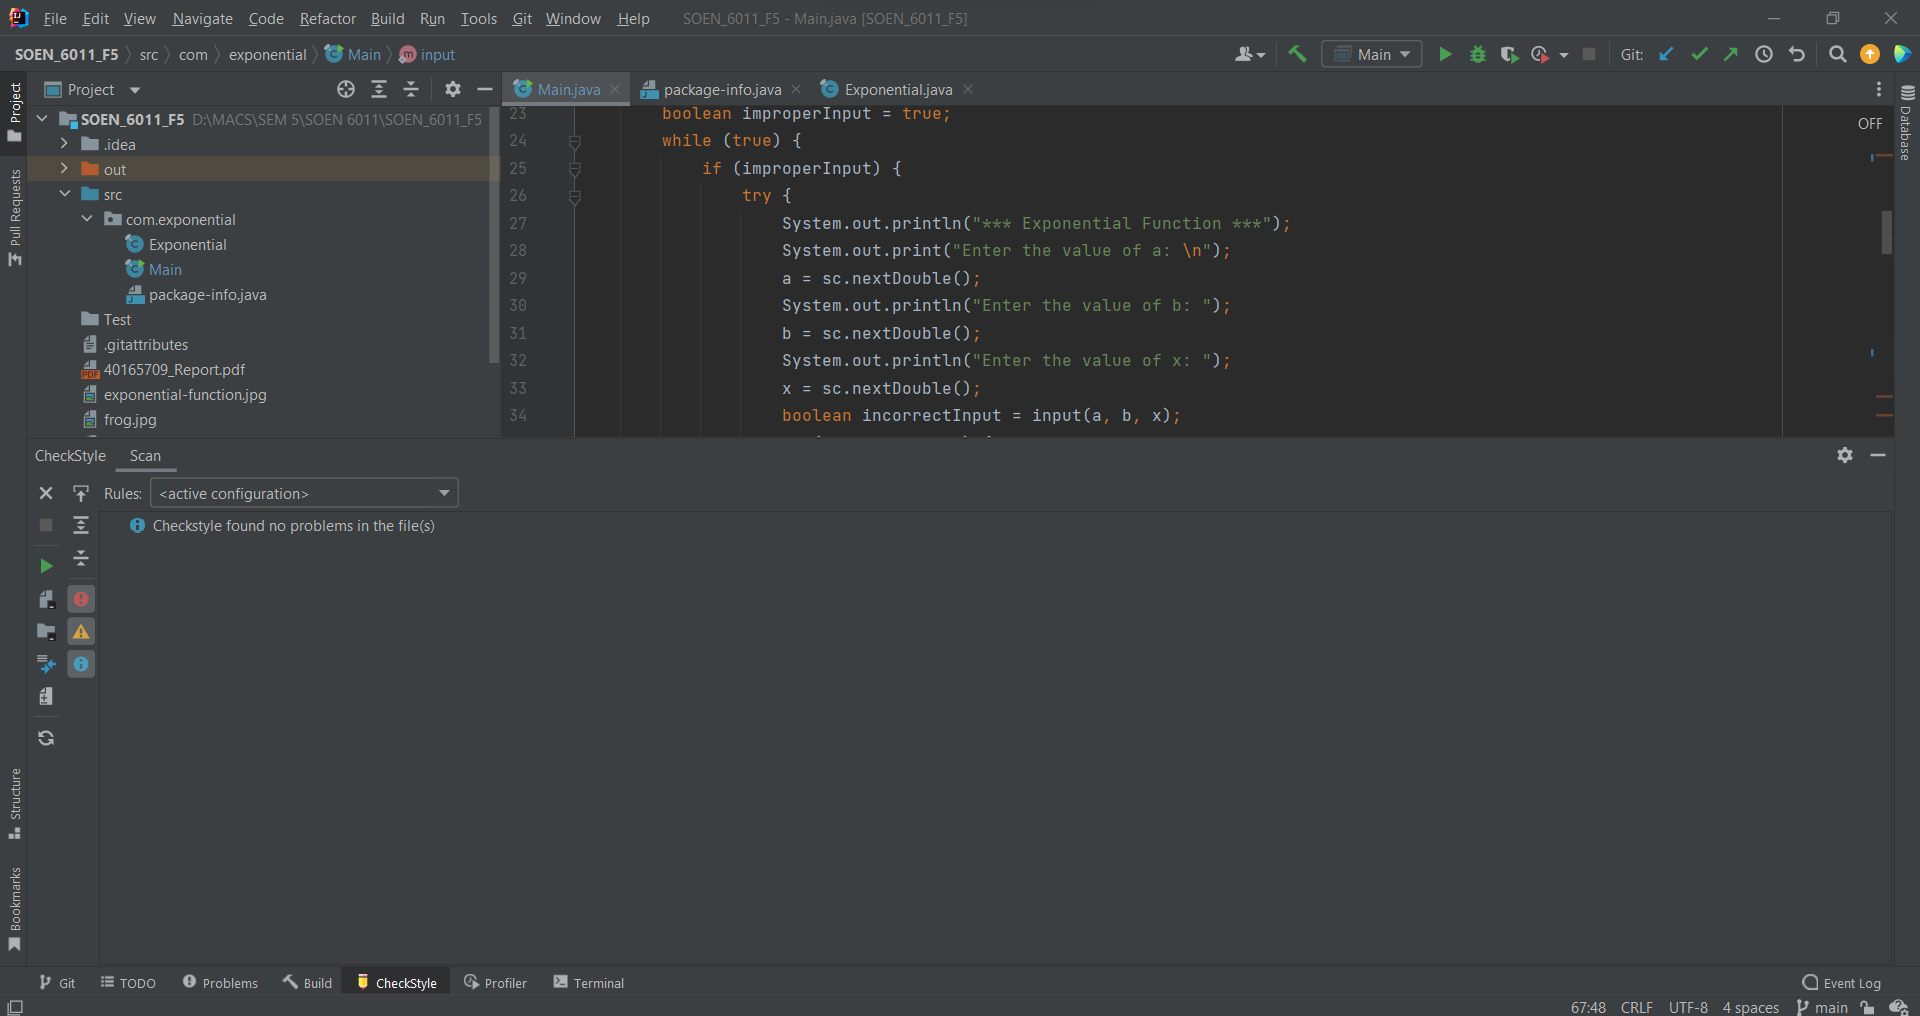
\includegraphics[width=15cm,height=9cm]{CheckStyle(After).png}
	\caption{Modified source code and resolved errors generated by Checkstyle tool}
	\label{Debugging computation of fractional exponent value}
\end{figure}

\newpage
\section{Problem 5 : Unit Test Cases }
In order to write unit tests for the function $ab^x$ , I have used \textbf{Junit 4} \cite{JUnit4} as the unit testing framework. I have designed various unit tests to test the successful functioning of the system as well as all the methods used in the program for certain computations, I have provided the tracing of the requirements with the designed unit tests along with the description as below.  
\newline
    
\noindent
\textbf{Requirement : }  REQ1 
\newline
\textbf{Unit Test : } testInvalidInputValueA()
\newline
\textbf{Description :} Tests' if the value of a and b are as required or else displays error message.
\newline
    
\noindent
\textbf{Requirement : }  REQ2
\newline
\textbf{Unit Test : } testInvalidInputValueB()
\newline
\textbf{Description :} Tests' if the value of b is non-negative or else displays error message.
\newline
    
\noindent
\textbf{Requirement : }  REQ3
\newline
\textbf{Unit Test : } testFunctionForValidInputs(), 
testFunctionForOddExponent(), \newline
testFunctionForEvenExponent(),
testFunctionForZeroValue()	
\newline
\textbf{Description :} All the unit tests, verifies the actual output and the result computed by the program for all valid inputs, with even and odd exponent as well as for zero value of exponent.
\newline
    
\noindent
\textbf{Requirement : }  REQ4
\newline
\textbf{Unit Test : } testFunctionForNegativeEvenExponent(), \newline
testFunctionForNegativeOddExponent(),
testFunctionForFractionalExponent(), \newline
testFunctionForNegativeFractionalExponent()
\newline
\textbf{Description :} All the unit tests, verifies the actual output and the result computed by the program for negative exponent as well as fractional exponent values.
\newline
     
\noindent
\textbf{Requirement : }  REQ5
\newline
\textbf{Unit Test : } testInvalidInputValue()
\newline
\textbf{Description : } Test if the input values are of the double type or else displays error message.
\newline
    
\noindent
\textbf{Requirement : }  REQ7
\newline
\textbf{Unit Test : } testFunctionCalculationTime()
\newline
\textbf{Description : } Test if the computation of the function is performed within the desired amount of time to meet the requirement.
    
\newpage
    
\begin{thebibliography}{20}
	\bibitem{Exponential Growth and Decay}
	Exponential Growth and Decay,\\
	https://virtuallearningacademy.net/VLA/LessonDisplay/Lesson6156/MATHAL GIIBU17Exponential\_Decay.html. Accessed 31 July 2022.
	
	\bibitem{Injectivity and Surjectivity of Exponential Function}
	Injectivity and Surjectivity of Exponential Function,\\
	https://math.stackexchange.com/q/349902. Accessed 31 July 2022
	
	
	\bibitem{Exponential Function Graph}
	Exponential Function Graph,\\
	https://www.basic-mathematics.com/exponential-function.html. Accessed 31 July 2022.
	
	\bibitem{Requirements Engineering}
	"ISO/IEC/IEEE International Standard - Systems and software engineering -- Life cycle processes -- Requirements engineering," in ISO/IEC/IEEE 29148:2018(E) , vol., no., pp.1-30, 30 Nov. 2018, doi: 10.1109/IEEESTD.2018.8559686.
	
	\bibitem{Pseudocode}
	Pseudocode,\\
	https://en.wikipedia.org/w/index.php?title=Pseudocode\&oldid=1101060705.  Accessed 31 July 2022
	
	\bibitem{Recursive Power Function}
	Power Function,\\
	https://afteracademy.com/blog/calculate-power-function. Accessed 31 July 2022.
	
	\bibitem{Algorithms}
	Algorithms,\\
	https://mathonweb.com/help\_ebook/html/algorithms.htm. Accessed 31 July 2022.
	
	\bibitem{Advantages and Disadvantages of Recursion}
	Advantages and Disadvantages of Recursion\\
	https://medium.com/@williambdale/recursion-the-pros-and-cons-76d32d75973a. Accessed 31 July 2022.
	 
	\bibitem{IntelliJ Debugger}
	IntelliJ Debugger,\\
	https://www.jetbrains.com/help/idea/debugging-code.html. Accessed 31 July 2022.
	
	\bibitem{Quality Assurance}
	Quality Assurance, Software Quality Attributes,\\
	http://www.qasigma.com/2008/12/software-quality-attributes.html. Accessed 31 July 2022.
	
	
	\bibitem{Checkstyle}
	Checkstyle – Checkstyle 10.3.1,\\
	https://checkstyle.sourceforge.io/. Accessed 31 July 2022.
	
	\bibitem{JUnit4}
	Junit 4,\\
	https://www.vogella.com/tutorials/JUnit4/article.html. Accessed 31 July 2022.
	
\end{thebibliography}

\newpage

\end{document}